\documentclass{book}
\usepackage[utf8]{vietnam}
\usepackage{cite}
\usepackage{amsmath,amssymb,amsfonts}
\usepackage{algorithm}
\usepackage{algorithmic}
\usepackage{graphicx}
\usepackage{textcomp}
\usepackage{xcolor}
\usepackage{tabularx}
\usepackage{listings}
\usepackage{enumerate}
\usepackage{fancyhdr}
\pagestyle{headings}

\fancyfoot[LE,RO]{Bản quyền thuộc Võ Thị Lưu Phương.}

\begin{document}

\title{TỐI ƯU LỒI VÀ ỨNG DỤNG TRONG MÁY HỌC}
\author{Võ Thị Lưu Phương}


\maketitle

\chapter{BÀI TOÁN QUY HOẠCH TUYẾN TÍNH}
\textit{Tác giả: Võ Thị Lưu Phương\\Email: vtlphuong@hcmiu.edu.vn}

\section{Giới thiệu bài toán quy hoạch tuyến tính}

Bài toán tối ưu tổng quát có dạng như sau:
\begin{align}
\rm{minimize}~  & f_0(x)\\
\rm{subject~to}~ &f_i(x) \leq b_i ,i=1,…,m.
\end{align}
Trong đó, vector $x=(x_1,\ldots,x_n)\in \mathbf{R}^n$ là biến số. Hàm $f_0(x)$ được gọi là hàm mục tiêu. Có $m$ ràng buộc trong bài toán tối ưu trên.  Ràng buộc thứ $i$ là $f_i(x) \leq b_i$.

Tối ưu hóa được áp dụng trong nhiều lĩnh vực như sản xuất, kinh tế, tài chính, điều khiển, thống kê, giao thông, v.v…. Ta có thể đưa một bài toán tối ưu bất kỳ về dạng như trên. Nếu bài toán tối ưu là tối đa hóa hàm mục tiêu $f_0(x)$, ví dụ tối đa hóa lợi nhuận, thì ta có thể thay hàm mục tiêu bằng  $min. -f_0(x)$. Các ràng buộc cũng có thể đưa về dạng như trên.

% Định nghĩa về tuyến tính, half-space,...

Một lĩnh vực quan trọng của tối ưu hóa, mà cụ thể hơn là tối ưu lồi là bài toán quy hoạch tuyến tính. Bài toán quy hoạch tuyến tính là một bài toán tối ưu trong đó các hàm mục tiêu và hàm ràng buộc $f_i(x),\ i=0,\ldots,m$ đếu có dạng tuyến tính:
\begin{align}
\rm{minimize}~   &c^Tx\\
\rm{subject~to}~ &a_i^Tx \leq b_i ,i=1,\ldots,\ m.
\end{align}
Ta cũng có thể biểu diễn ràng buộc dạng ma trận $Ax \leq b$, trong đó $c,a_1,\ldots,a_m \in \mathbf{R}^n$, $A=\left[\begin{matrix}a_1^T\\
\ldots\\a_m^T
\end{matrix}\right]$, và $b=\left[\begin{matrix}b_1\\
\ldots\\
b_m
\end{matrix}\right]$.


Sau đây là vài ví dụ về bài toán quy hoạch tuyến tính.
\subsubsection{Ví dụ 1}
\begin{align}
\rm{min.}~ & f = x_1+x_2 	\label{eq:chap1_ex1}\\
\rm{s.t.}~ & x_1+2x_2\geq 2,\nonumber\\
	& 3x_1+x_2\geq 2,\nonumber\\
	&	x_1 \geq 1,\nonumber\\ 
	&	x_2 \geq 0.	\nonumber	
\end{align}

Hình 1.1 mô tả hàm mục tiêu và miền khả thi (feasible region) của bài toán trên giúp bạn đọc có cảm giác về nghiệm của bài toán tối ưu.
\begin{figure}[h]
	\centering
	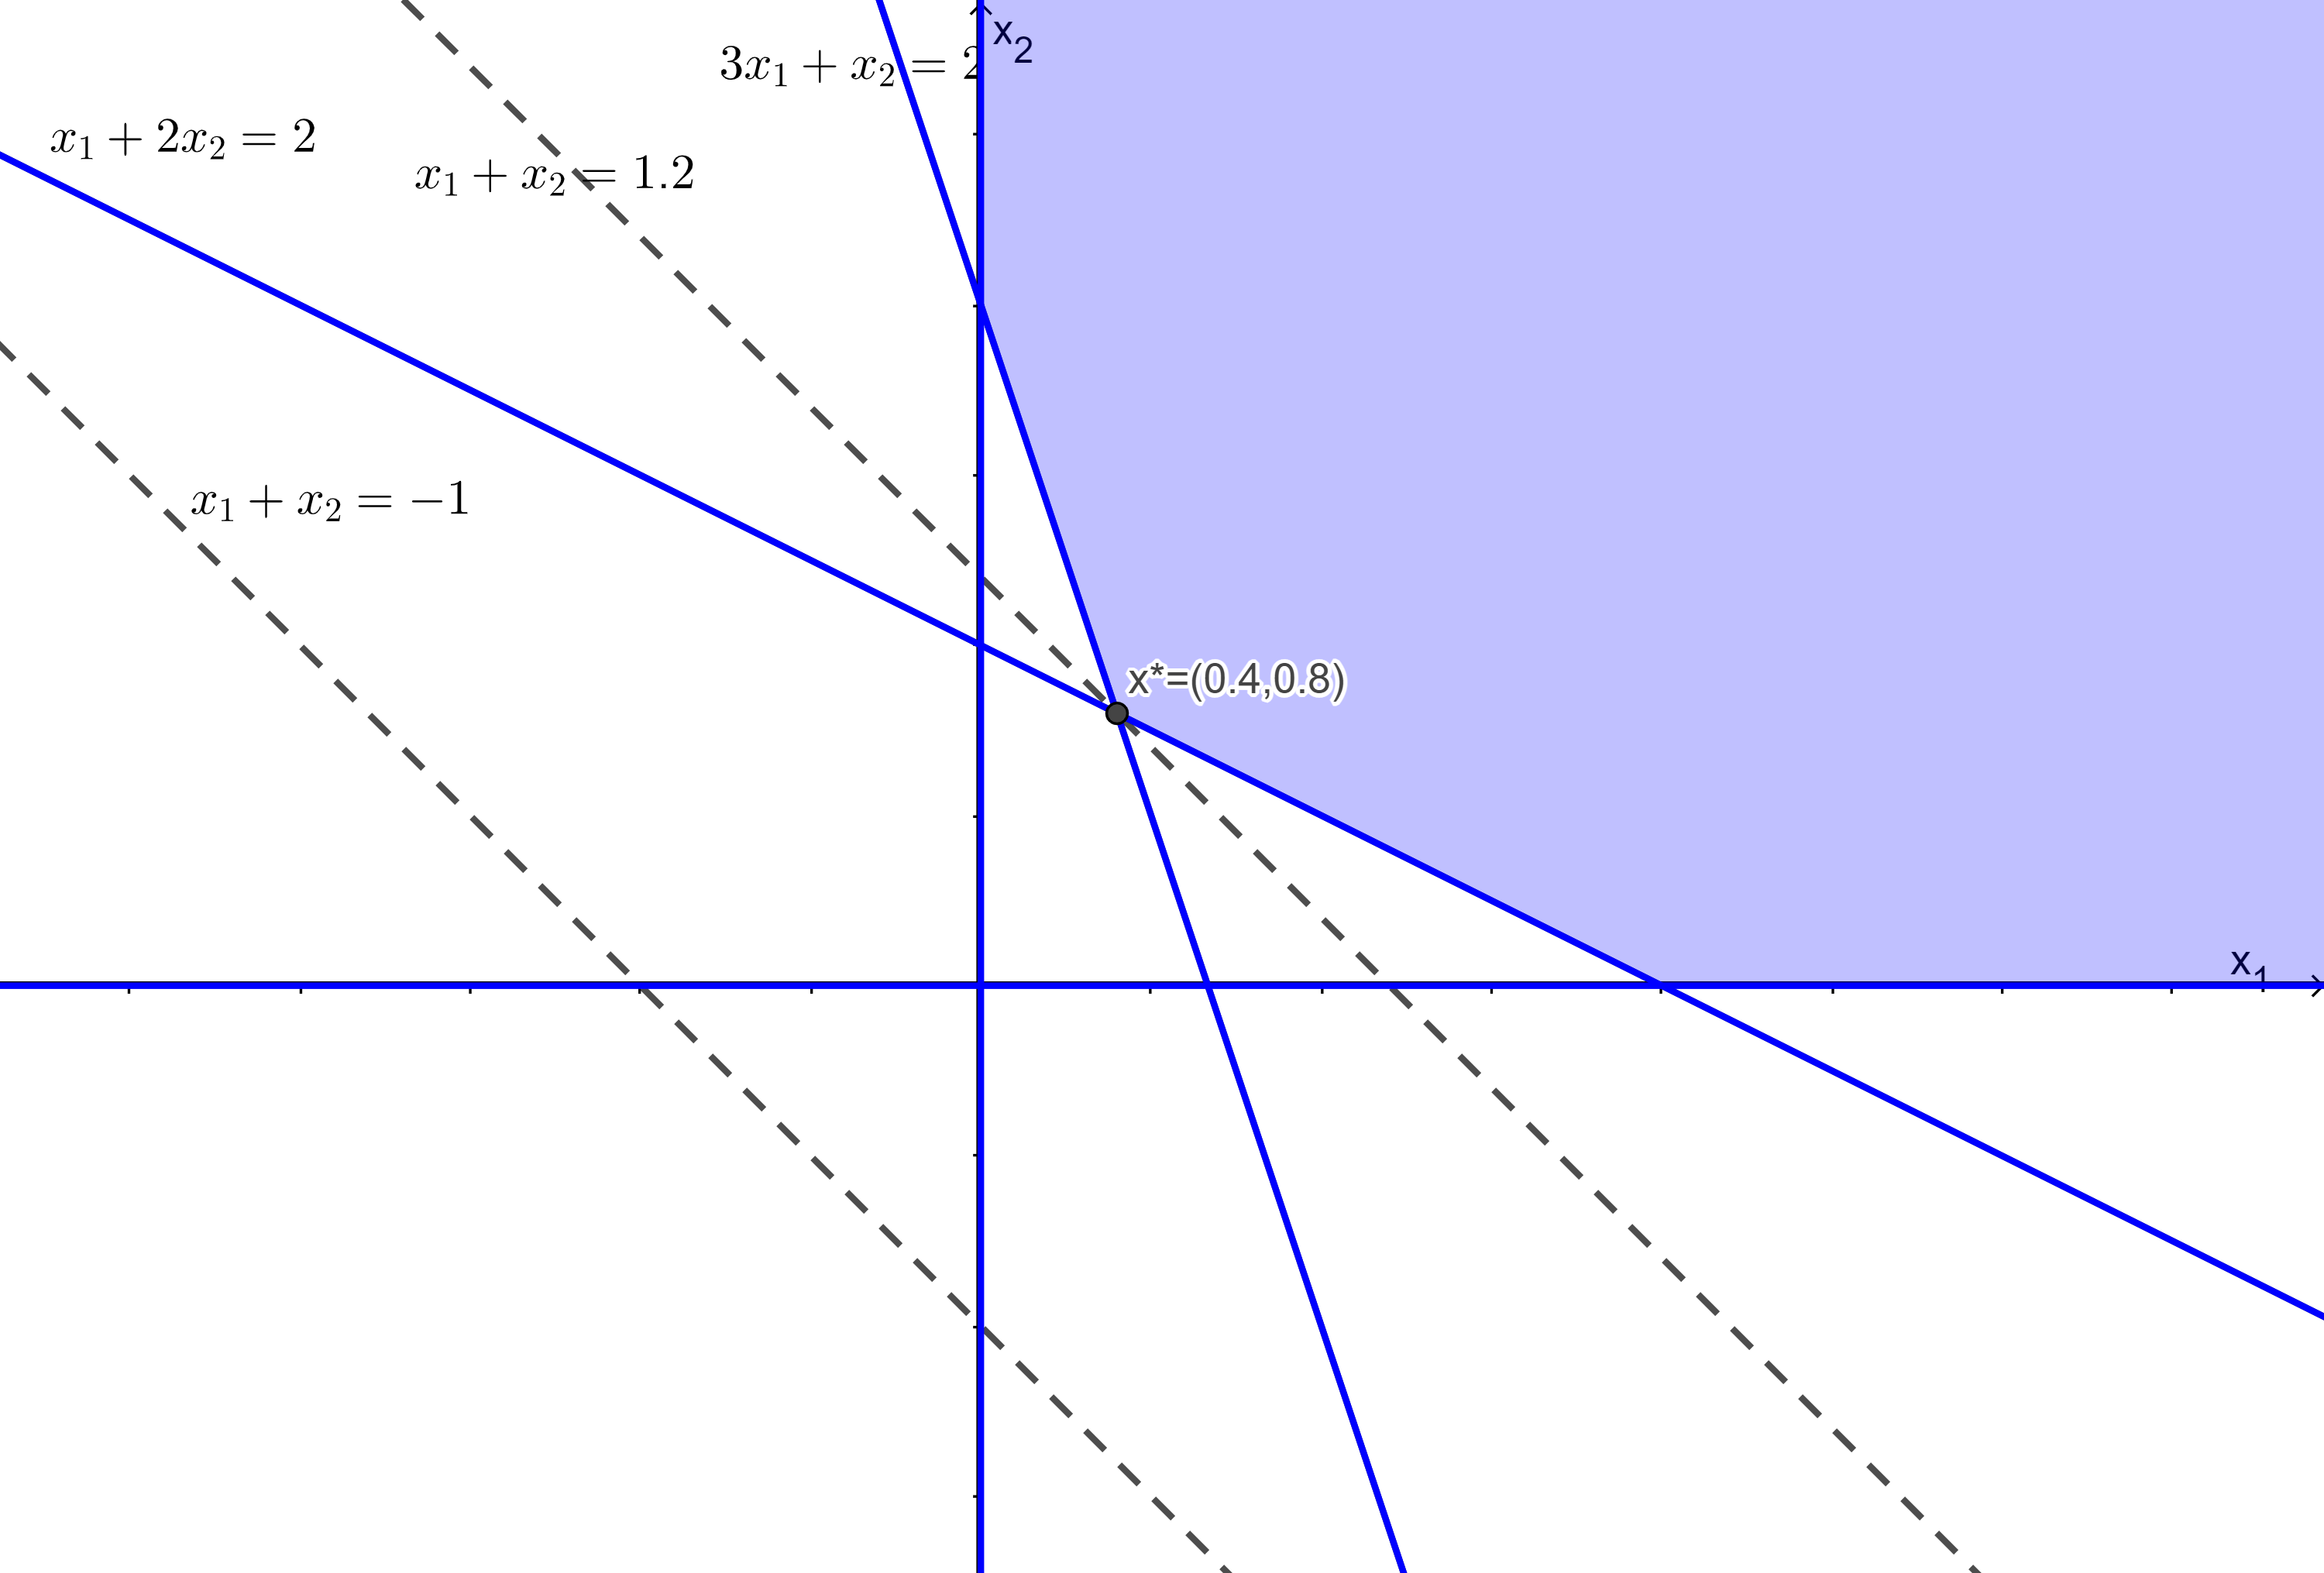
\includegraphics[width=9.5cm]{hinh_chuong1_lp/chap1_ex1.png}
	\caption{Biểu diễn hình học của hàm mục tiêu và các ràng buộc. Vùng tô màu là miền khả thi của bài toán trong ví dụ \eqref{eq:chap1_ex1}.
	Nghiệm tối ưu là $f^* = 1.2$, đạt được tại vector $x^*=(0.4,0.8)$.}
	\label{fig:vidu1.1}	
\end{figure}


Trong các sách về quy hoạch tuyến tính truyền thống mà giải thuật đơn hình (simplex) được giới thiệu như một phương pháp chính để giải bài toán, bài toán LP được giới thiệu ở dạng chính tắc như sau:
\begin{align}
\rm{maximize}~   &c^Tx\\
\rm{subject~to}~ &a_i^Tx \leq b_i ,i=1,\ldots,\ m\\
				& x \geq 0.
\label{eq-standardLP}
\end{align}
Bài toán dạng chính tắc là đầu vào của giải thuật đơn hình.

Thực ra, ta có thể biến đổi một bài toán LP bất kỳ về dạng chính tắc \eqref{eq-standardLP}, ví dụ như:
\begin{itemize}
\item Nếu hàm mục tiêu là $\rm{min.}~c^Tx$ thì có thể thay bằng $\rm{max.}~ -c^Tx$.
\item Nếu ràng buộc là $a_i^Tx \geq b_i$ thì có thể thay bằng $-a_i^Tx \leq -b_i$.
\item Nếu ràng buộc là $a_i^Tx = b_i$ thì có thể thay bằng hai ràng buộc tương đương: $a_i^Tx \geq b_i$ và $a_i^Tx \leq b_i$.
\item Nếu không có ràng buộc $x_i \geq 0$ thì có thể thay biến $x_i = x_i^+ - x_i^-$, trong đó $x_i^+, x_i^- \geq 0$.
\end{itemize}

\subsubsection{Ví dụ 2 - Bài toán dinh dưỡng}
Để đảm bảo được dinh dưỡng, một người trung bình cần cho mỗi ngày:
\begin{itemize}
\item	Không ít hơn 200 gam chất bột đường (carbohydrate)
\item	Không ít hơn 20 gam chất đạm (protein)
\end{itemize}
Hàm lượng dinh dưỡng các chất này trong 04 loại lương thực hiện có trong một cửa hàng trong 1000 gram được liệt kê ở bảng sau:\\
\begin{tabular}{|c|c|c|c|}
\hline
Loại thức ăn	& bột đường	(gram) &đạm (gram)	&giá (ngàn đồng)\\
\hline
Cà rốt	&300	&30	&50\\
\hline
Gạo		&400	&10	&20\\
\hline
Khoai tây	&400	&20	&10\\
\hline
Bột mì	&500	&50	&30\\
\hline
\end{tabular}

\textit{Ghi chú: các số liệu trên chỉ dùng để minh họa cho ví dụ.}

Như vậy người đó cần tối thiểu là bao nhiêu tiền đề đảm bảo được dinh dưỡng cho bữa ăn.
Bài toán dinh dưỡng được mô hình dưới dạng bài toán quy doạch tuyến tính như sau:
Gọi $x_c, x_g, x_k, x_b$ là số gram cà rốt, gạo, khoai tây và bột mì cần mua. 
Hàm mục tiêu là tổng số tiền:
\begin{align}
50x_c+20x_g+10x_k+30x_b
\end{align}
Các ràng buộc bao gồm:
\begin{itemize}
\item Đảm bảo về hàm lượng bột đường:
\begin{align}
300x_c+400x_g+400x_k+500x_b \geq 200
\end{align}
\item Đảm bảo về hàm lượng đạm:
\begin{align}
30x_c+10x_g+20x_k+50x_b\geq20
\end{align}

\item Ngoài ra còn có ràng buộc không âm cho các biến:
$x_c\geq0,\ x_g \geq 0,x_k \geq 0,x_b\geq0$.
\end{itemize}

Như vậy, bài toán quy hoạch tuyến tính cho dinh dưỡng sẽ là:
\begin{align}
min.~& 50x_c+20x_g+10x_k+30x_b \\
s.t.~ & 300x_c+400x_g+400x_k+500x_b\geq200,\\
	&	30x_c+10x_g+20x_k+50x_b\geq20,\\ 
	&	x_c\geq0,\ x_g\geq0,x_k\geq0,x_b\geq0.		
\end{align}
%với biến $x=\left[x_c,\ x_g,x_k,x_b\right]^T,x\in \mathbf{R}^4$, 
%$A=\begin{bmatrix}
%300 & 400 & 400 & 500
%\end{bmatrix}$
%viết theo dạng ma trận

\subsubsection{Giải bài toán quy hoạch tuyến tính bằng CVXPY solver}
Có nhiều thư viện cho phép giải một bài toán quy hoạch tuyến tính. Sách này xin giới thiệu thư viện CVXPY dùng trong ngôn ngữ Python.
 
\begin{lstlisting}[frame=single]
import cvxpy as cp
import numpy as np

c = np.array([5, 2, 1, 10])
A = np.array([[50, 40,40, 40],[3, 1, 2, 5]])
b = np.array([200, 20])

x = cp.Variable(4)
constraint = [A@x >= b, x >=0]
prob = cp.Problem(cp.Minimize(c.T@x), constraint)
prob.solve()

# Print result.
print("\nThe optimal value is", prob.value)
print("A solution x is")
print(x.value)

\end{lstlisting}

\subsubsection{Nghiệm của bài toán LP}
Một bài toán LP có thể có 3 loại nghiệm:
\begin{itemize}
\item Bài toán có nghiệm hữu hạn: ví dụ như bài toán được cho trong ví dụ 1.1\eqref{eq:chap1_ex1} trên.

\item Bài toán vô nghiệm:
Một bài toán LP là vô nghiệm khi miền khả thi không tồn tại.
Ví dụ bài toán sau là vô nghiệm
	\begin{align*}
		\rm{min.}~ & x_1+x_2 \\
		\rm{s.t.}~ & x_1-2x_2 \geq 2,\\
			&	x_1 \geq 0,\\ 
			&	x_1 \leq -3.		
	\end{align*}
Không tồn tại miền khả thi đồng thời thỏa cả hai ràng buộc $x_1 >=0$ và $x_1 <= -3$.

\item Bài toán có nghiệm vô cực:
Ví dụ bài toán sau là vô nghiệm
	\begin{align*}
		\rm{min.}~ & -x_1+2x_2 \\
		\rm{s.t.}~ & x_1 \leq 3,\\
			&	x_2 \geq 7,\\ 
			&	-x_1+2x_2 \leq -5.		
	\end{align*}
\end{itemize}

\section{Bài toán LP đối ngẫu}
Bài toán đối ngẫu là một chủ đề rất quan trọng trong tối ưu. 
Nhiều lúc thay vì giải bài toán gốc, xem xét bài toán đối ngẫu giúp ta hiểu được các bản chất đằng sau của hàm mục tiêu, các ràng buộc. Ví dụ trong phương pháp dual decomposition, thay vì giải bài toán gốc là bài toán lớn, không thể giải được thì phương pháp này phân rã bài toán đối ngẫu ra thành nhiều bài toán con với kích thước nhỏ hơn và giải song song đồng thời. 
Trong phần này, bài toán đối ngẫu của LP được giới thiệu sơ lược để giúp bạn đọc có một cái nhìn trực quan. 
Lý thuyết đối ngẫu sẽ được giới thiệu kỹ sau này trong phần tối ưu lồi.

Xét bài toán LP sau
\begin{align}
\rm{min.}~ & f(x_1, x_2) = x_1 + x_2 \label{eq-ex13-obj}\\
\rm{s.t.}~ & x_1 - 2x_2 \geq -1,\label{eq-ex13-c1}\\
		& - 2x_1 + x_2 \geq 1,\label{eq-ex13-c2}\\
		&  x_1 + 4x_2 \geq 6 \label{eq-ex13-c3}\\
		&	x_1 \geq 0,	x_2 \geq 0.		
\end{align}
Bây giờ ta tìm hiểu chặn trên và chặn dưới của nghiệm bài toán.
Đối với bài toán tìm cực tiểu, chặn trên là bất cứ điểm nào thuộc miền khả thi.
Gọi $x_1, x_2$ là một điểm thỏa mãn các ràng buộc, ta luôn có $f(x_1, x_2) \leq f(x_1^*, x_2^*)$.

Bây giờ để tìm chặn dưới của nghiệm, ta nhân hai vế của các điều kiện  \eqref{eq-ex13-c1}, \eqref{eq-ex13-c2}, và \eqref{eq-ex13-c3} với ba số không âm tương ứng là $\lambda_1$, $\lambda_2$, và $\lambda_3$, ta được các ràng buộc mới tương đương.
\begin{align*}
 \lambda_1 x_1 - 2\lambda_1 x_2 &\geq -\lambda_1,\\
 - 2\lambda_2 x_1 + \lambda_2 x_2 &\geq \lambda_2,\\
  \lambda_3 x_1 + 4\lambda_3 x_2 &\geq 6\lambda_3.\\
\end{align*}

Cộng ba ràng buộc mới với nhau vế theo vế, ta được 
\begin{align*}
(\lambda_1 -2 \lambda_2 + \lambda_3)x_1 + (- 2 \lambda_1 + \lambda_2 + \lambda_3)x_2 \geq -\lambda_1 +  \lambda_2 + 6\lambda_3.
\end{align*}
Nếu tồn tại $\lambda_1, \lambda_2 \geq 0$ sao cho 
\begin{align*}
\lambda_1 -2 \lambda_2 + \lambda_3 		&\leq 1 \\
- 2 \lambda_1 + \lambda_2 + \lambda_3 	&\leq 1.
\end{align*}
thì ta có 
\begin{align*}
-\lambda_1 +  \lambda_2 + 6\lambda_3 & \geq (\lambda_1 -2 \lambda_2 + \lambda_3)x_1 + (- 2 \lambda_1 + \lambda_2 + \lambda_3)x_2 \\
 									& \geq x_1+	x_2 = f.
\end{align*}
Như vậy, $-\lambda_1 +  \lambda_2 + 6\lambda_3$ là một chặn dưới của bài toán.

Một câu hỏi được đặt ra là với những giá trị $\lambda_1, \lambda_2, \lambda_3$ nào thì ta có chặn dưới là tốt nhất. 
Đó chính là bài toán đối ngẫu của bài toán \eqref{eq-ex13-obj}:
\begin{align*}
\rm{min.}~ & -\lambda_1 +  \lambda_2 + 6\lambda_3\\
\rm{s.t.}~ & \lambda_1 -2 \lambda_2 + \lambda_3 \geq 1 \\
		& - 2 \lambda_1 + \lambda_2 + \lambda_3 \geq 1,\\
		&	\lambda_1,	\lambda_2, \lambda_3 \geq 0.		
\end{align*}

Đối với bài toán LP tổng quát
\begin{align*}
\rm{min.}~ & c^Tx = c_1 x_1 + \ldots + c_2 x_2 \\
\rm{s.t.}~ & a_{j1}x_1+ \ldots + a_{jn}x_n \geq b_j, j=1,\ldots, m\\
		&	x_1, \ldots, x_n \geq 0.
\end{align*}
thì bài toán đối ngẫu sẽ có dạng
\begin{align*}
\rm{max.}~ & b^T \lambda = b_1 \lambda_1 + \ldots + b_m \lambda_m \\
\rm{s.t.}~ & a_{1j}\lambda_1+ \ldots + a_{nj}\lambda_n \leq c_j, j=1,\ldots, m\\
		&	\lambda_1, \ldots, \lambda_m \geq 0.
\end{align*}

Một tính chất đối ngẫu quan trọng là nghiệm của bài toán LP đối ngẫu cũng là nghiệm của bài toán LP gốc. Do đó, thay vì giải bài toán gốc, ta có thể giải bài toán đối ngẫu.
Chương sau sẽ đề cập chi tiết hơn đến lý thuyết đối ngẫu cho một bài toán tối ưu dạng tổng quát.

%\section{Một số bài toán ứng dụng quy hoạch tuyến tính}


\section{Bài tập}
\begin{enumerate}
\item Biểu diễn các bài toán LP sau dưới dạng vector và ma trận. Bài toán là vô nghiệm, nghiệm vô cùng hay tồn tại nghiệm hữu hạn? Giải thích bằng biểu diễn trên đồ thị 2D? Giải bài toán bằng thư viện CVXPY để so sánh hai kết quả?
	\begin{enumerate}[a.]
	\item 
	\begin{align*}
		\rm{min.}~ & x_1+x_2 \\
		\rm{s.t.}~ & x_1-2x_2 \geq 2,\\
			&	x_1 \geq 0,\\ 
			&	x_2 \geq 0.		
	\end{align*}
	
	\item 
	\begin{align*}
		\rm{min.}~ & x_1-x_2 \\
		\rm{s.t.}~ & x_1+2x_2 \leq -1,\\
			&	x_2 \geq 3.		
	\end{align*}
	
	\item 
	\begin{align*}
		\rm{max.}~ & x_1-x_2 \\
		\rm{s.t.}~ & 3x_1+x_2 \leq 3,\\
			&	x_1+x_2 \geq 1\\	
			&	x_2 \geq 3.		
	\end{align*}
	\end{enumerate}
\end{enumerate}

\section{Ghi chú}
Thuật ngữ tuyến tính được dịch từ chữ linear hoặc affine trong tiếng Anh. Thực ra có sự khác nhau nhỏ giữa linear và affine. Một hàm $f(x) = a^Tx+b$ được gọi là affine, trong khi hàm $f(x) = a^Tx$ được gọi linear. Một hàm linear là affine, nhưng ngược lại thì không đúng. Sách này đề cập hàm tuyến tính tức là hàm affine.

Có nhiều nguồn tài liệu cho phép người học làm quen với ngôn ngữ Python, ví dụ \cite{pythonbook}.
Các bài tập trong chương này được tham khảo từ các sách \cite{Vanderbei, Boyd}

\begin{thebibliography}{8}
\bibitem{Boyd}
Boyd, Stephen, Stephen P. Boyd, and Lieven Vandenberghe. Convex optimization. Cambridge university press, 2004.

\bibitem{Vanderbei}
Vanderbei, Robert J. Linear programming: foundations and extensions. Vol. 285. Springer Nature, 2020.


\bibitem{pythonbook}
Wentworth, Peter, Jeffrey Elkner, Allen B. Downey, and Chris Meyer. How to think like a computer scientist: Learning with Python 3. (2015).

\end{thebibliography}

\end{document}